\section{Durchführung}
\label{sec:Durchführung}
\begin{figure}[H]
  \centering
  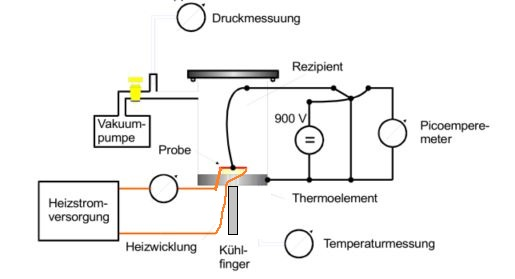
\includegraphics{plots/Aufbau.JPG}
  \caption{Versuchsaufbau zur Messung der Spannung und Temperatur.\cite{Anleitung}}
  \label{fig:aufbau}
\end{figure}
Der Aufbau der Messapparatur ist in Abbildung \ref{fig:aufbau} zu sehen. Bevor mit der Messung begonnen werden kann, wird der
Probenbehälter bis zu einem Unterdruck von ca. $\SI{e-2}{\milli\bar}$ evakuiert. Gleichzeitig wird bei maximaler Heizspannung
die Probe bis auf $\SI{333}{\kelvin}$ aufgeheizt. Währendessen wird der Kondensator angeschlossen und bei einer Spannung von
$\SI{950}{\volt}$ über ungefähr $\SI{900}{\second}$ eingeschaltet.\\
Anschließend wird bei eingeschaltetem Kondensator die Probe mittels flüssigem Stickstoff auf $\SI{210}{\kelvin}$ abgekühlt.
Jetzt wird der Kondensator kurzgeschlossen und anschließend das Picoamperemeter angeschlossen. Die gekühlte Probe wird nun bei einer Heizrate $H_1$ wieder bis auf $\SI{333}{\kelvin}$ aufgeheizt.
Währendessen werden für Temperatur und Depolarisationsstrom pro Minute ein Wertepaar aufgenommen. Der Messvorgang wird ein zweites Mal bei einer zweiten Heizrate $H_2$ ausgeführt.
